\documentclass[11pt]{article}

\usepackage{latexsym}
\usepackage{amsmath}
\usepackage{amssymb}
\usepackage{amsthm}
\usepackage{graphicx}
\usepackage{wrapfig}
\usepackage{pseudocode}
\usepackage{url}
\usepackage[backref, colorlinks=true, citecolor=red, urlcolor=blue, pdfauthor={Jyh-Ming Lien}]{hyperref}


\newcommand{\handout}[5]{
  \noindent
  \begin{center}
  \framebox{
    \vbox{
      \hbox to 5.78in { {\bf } \hfill #2 }
      \vspace{4mm}
      \hbox to 5.78in { {\Large \hfill #5  \hfill} }
      \vspace{2mm}
      \hbox to 5.78in { {\em #3 \hfill #4} }
    }
  }
  \end{center}
  \vspace*{4mm}
}

\newcommand{\lecture}[4]{\handout{#1}{#2}{#3}{}{Report for #1}}

\newtheorem{theorem}{Theorem}
\newtheorem{corollary}[theorem]{Corollary}
\newtheorem{lemma}[theorem]{Lemma}
\newtheorem{observation}[theorem]{Observation}
\newtheorem{proposition}[theorem]{Proposition}
\newtheorem{definition}[theorem]{Definition}
\newtheorem{claim}[theorem]{Claim}
\newtheorem{fact}[theorem]{Fact}
\newtheorem{assumption}[theorem]{Assumption}

% 1-inch margins, from fullpage.sty by H.Partl, Version 2, Dec. 15, 1988.
\topmargin 0pt
\advance \topmargin by -\headheight
\advance \topmargin by -\headsep
\textheight 8.9in
\oddsidemargin 0pt
\evensidemargin \oddsidemargin
\marginparwidth 0.5in
\textwidth 6.5in

\parindent 0in
\parskip 1.5ex
%\renewcommand{\baselinestretch}{1.25}

\begin{document}

\lecture{Advance Algorithm Programming Assignment 1 Part2 }{Fall 2015}{Moran Kim}


\section{Implementation Details}
Given N number of points in $\mathbb{R}^3 \hspace{0.15cm}$ to get a 3D $\alpha$-shape we need to compute the radius of circumsphere of Delaunay triangulation. By mathematical proof we know the center of the circumsphere of Delaunay triangulation is the voronoi vertex. We can get the vornoi vertex(center) by using qh.setvoronoi.all() (I used dot . instead of bottom dash line) as implemented in $"alpha-shape.c"$. From the tetrahedrons we obtained from Delaunay triangulation, we check whether the radius of circumsphere of each tetrahedron is less than $\alpha$ or not. \\
(1)Tetra part: By reporting only the vertices of tetrahedron whose radius of circumsphere is less than alpha.\\
(2)Face  part: By reporting only the vertices of tetrahedron which satisfies \\
   \begin{itemize}
     \item whose radius of circumsphere is less than alpha. [1]
     \item whose neighbor is upper Delaunay or whose radius of neighbor circumsphere is greater than alpha. [2]
   \end{itemize}
   if vertices satisfy [1] and [2], then report them to the vertex information.\\
(3)Edge  part: By reporting only the vertices of the tetrahedron which is obtained from(1).\\
If we give $\alpha=\infty$ then the shape will be the convex hull of given data set. As we use smaller value of $\alpha$, we will obtain more accurate 3D shape which close to the given set of points. If we give $\alpha=0$, the shape will be exactly same as the data points.\\
(In the code you can find a reference in every line )
\section{Example Output}
I tried the spoon and bb which are in the given data. When I tried spoon for $\alpha=100000$(Fig.1) there was not much difference in $\alpha=0$ and that means the distance between the set of points are really huge. So when I gave $\alpha=10000000$ I obtained the pictures below. The smaller value we give to $\alpha$ the more elaborately carved one we can see.

\begin{figure}[h]
  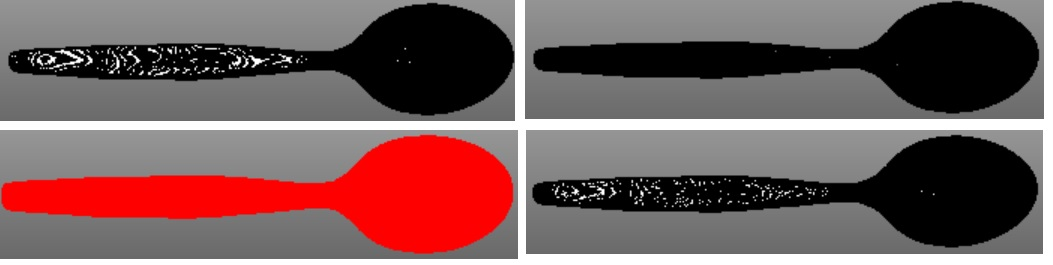
\includegraphics[width=120mm]{spoon 10000.jpg}\\
  Fig 1. $\alpha=100000\hspace{0.15cm}$facets, edges, points and tetrahedra (order from left to right, top to bottom)
\end{figure}

\begin{figure}[h]
  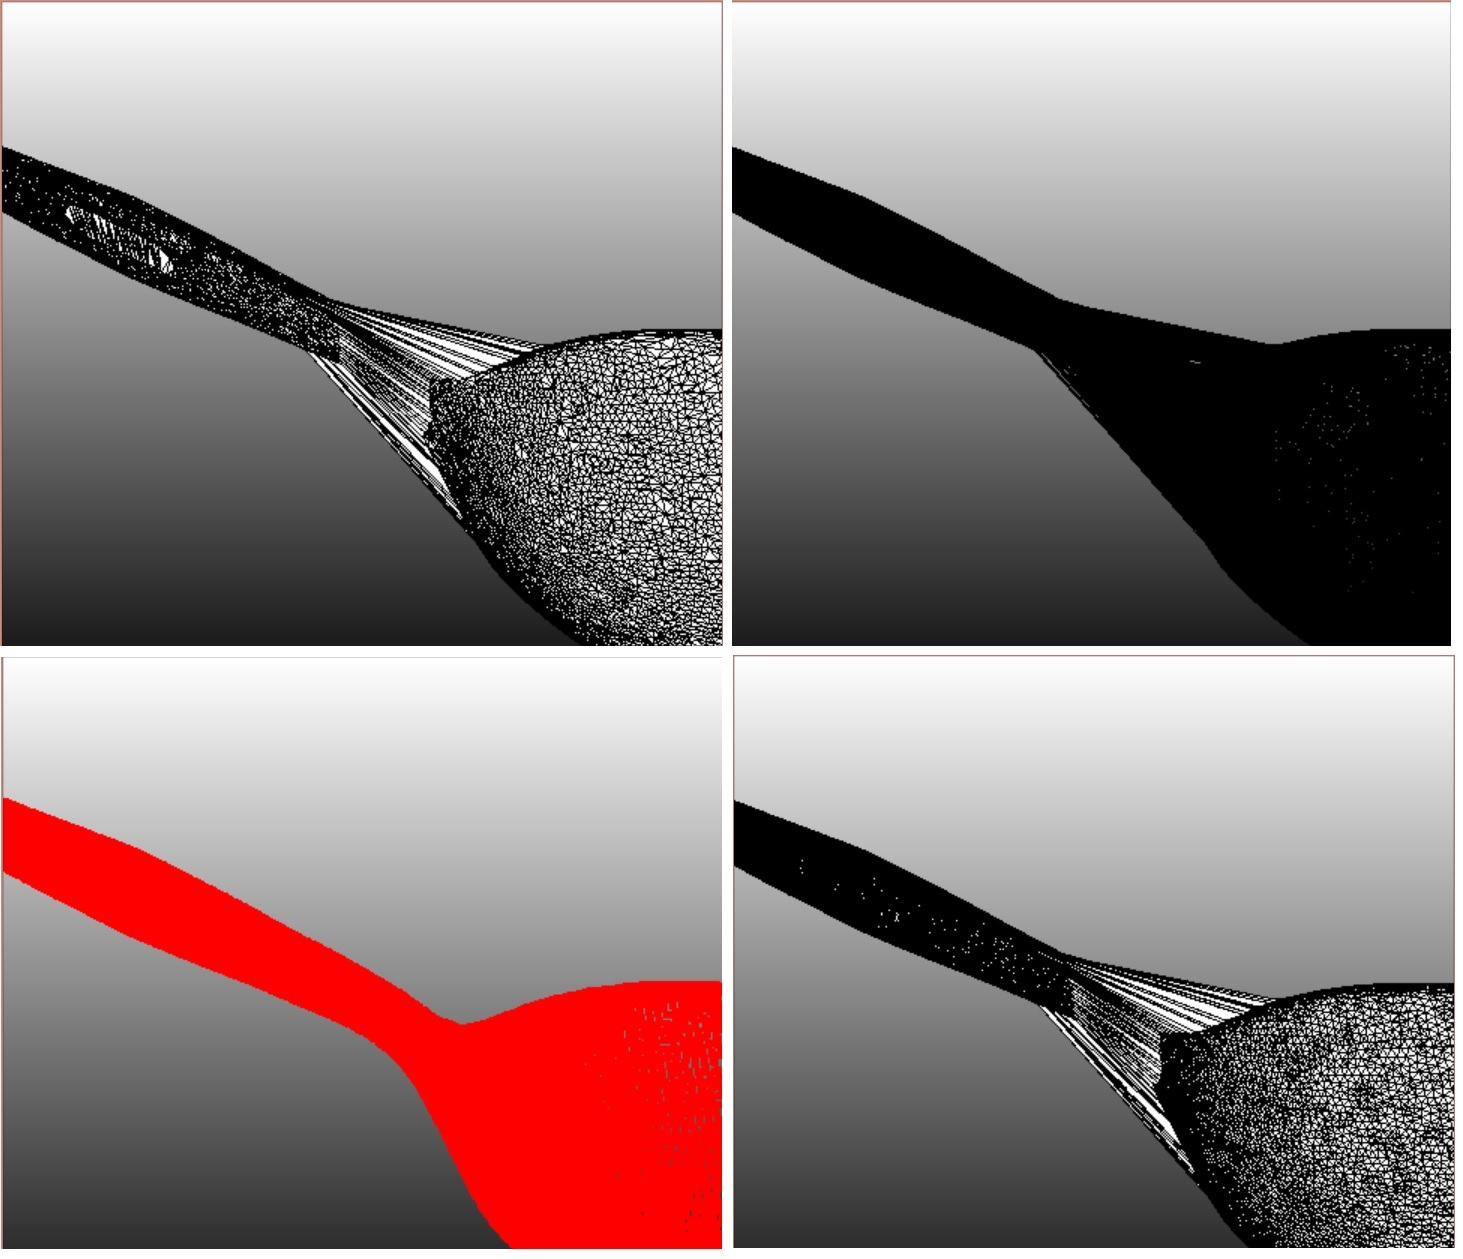
\includegraphics[width=120mm]{spoon 10000000.jpg}\\
  Fig 2. $\alpha=10000000\hspace{0.15cm}$facets, edges, points and tetrahedra
\end{figure}


\begin{figure}[h]
  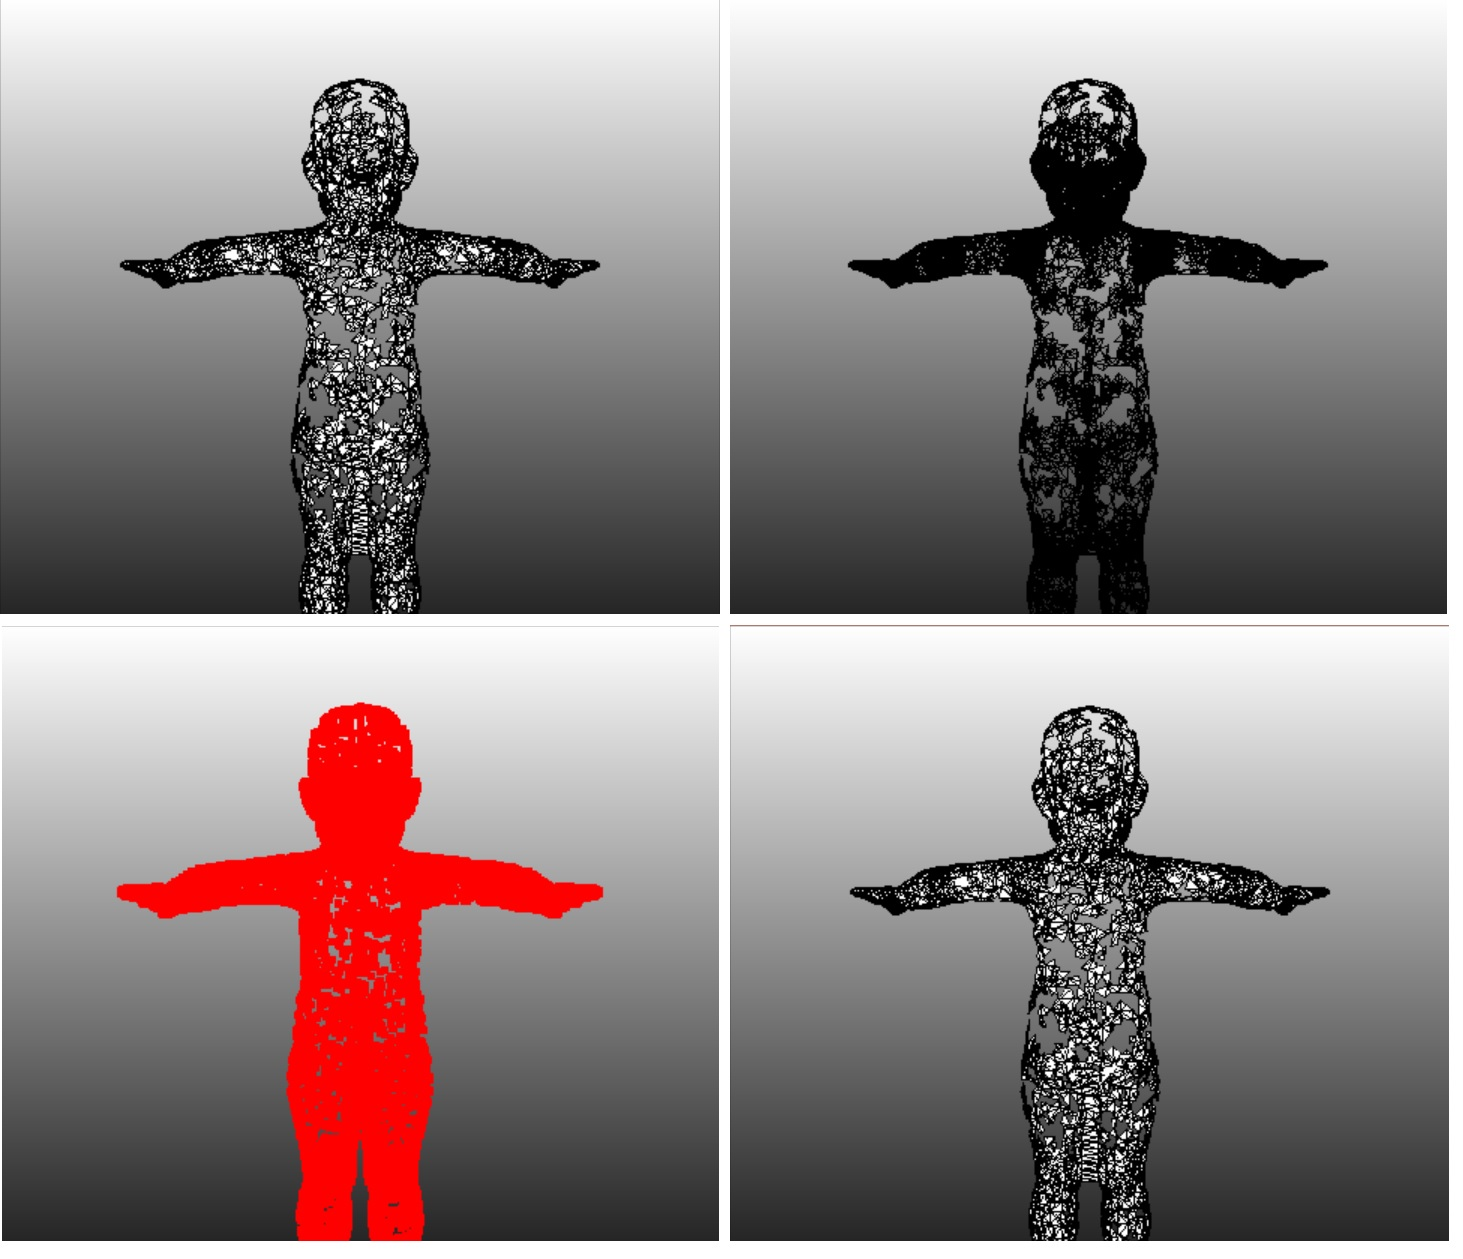
\includegraphics[width=120mm]{bb 30.jpg}\\
  Fig 3. $\alpha=30\hspace{0.15cm}$facets, edges, points and tetrahedra
\end{figure}


\begin{figure}[h]
  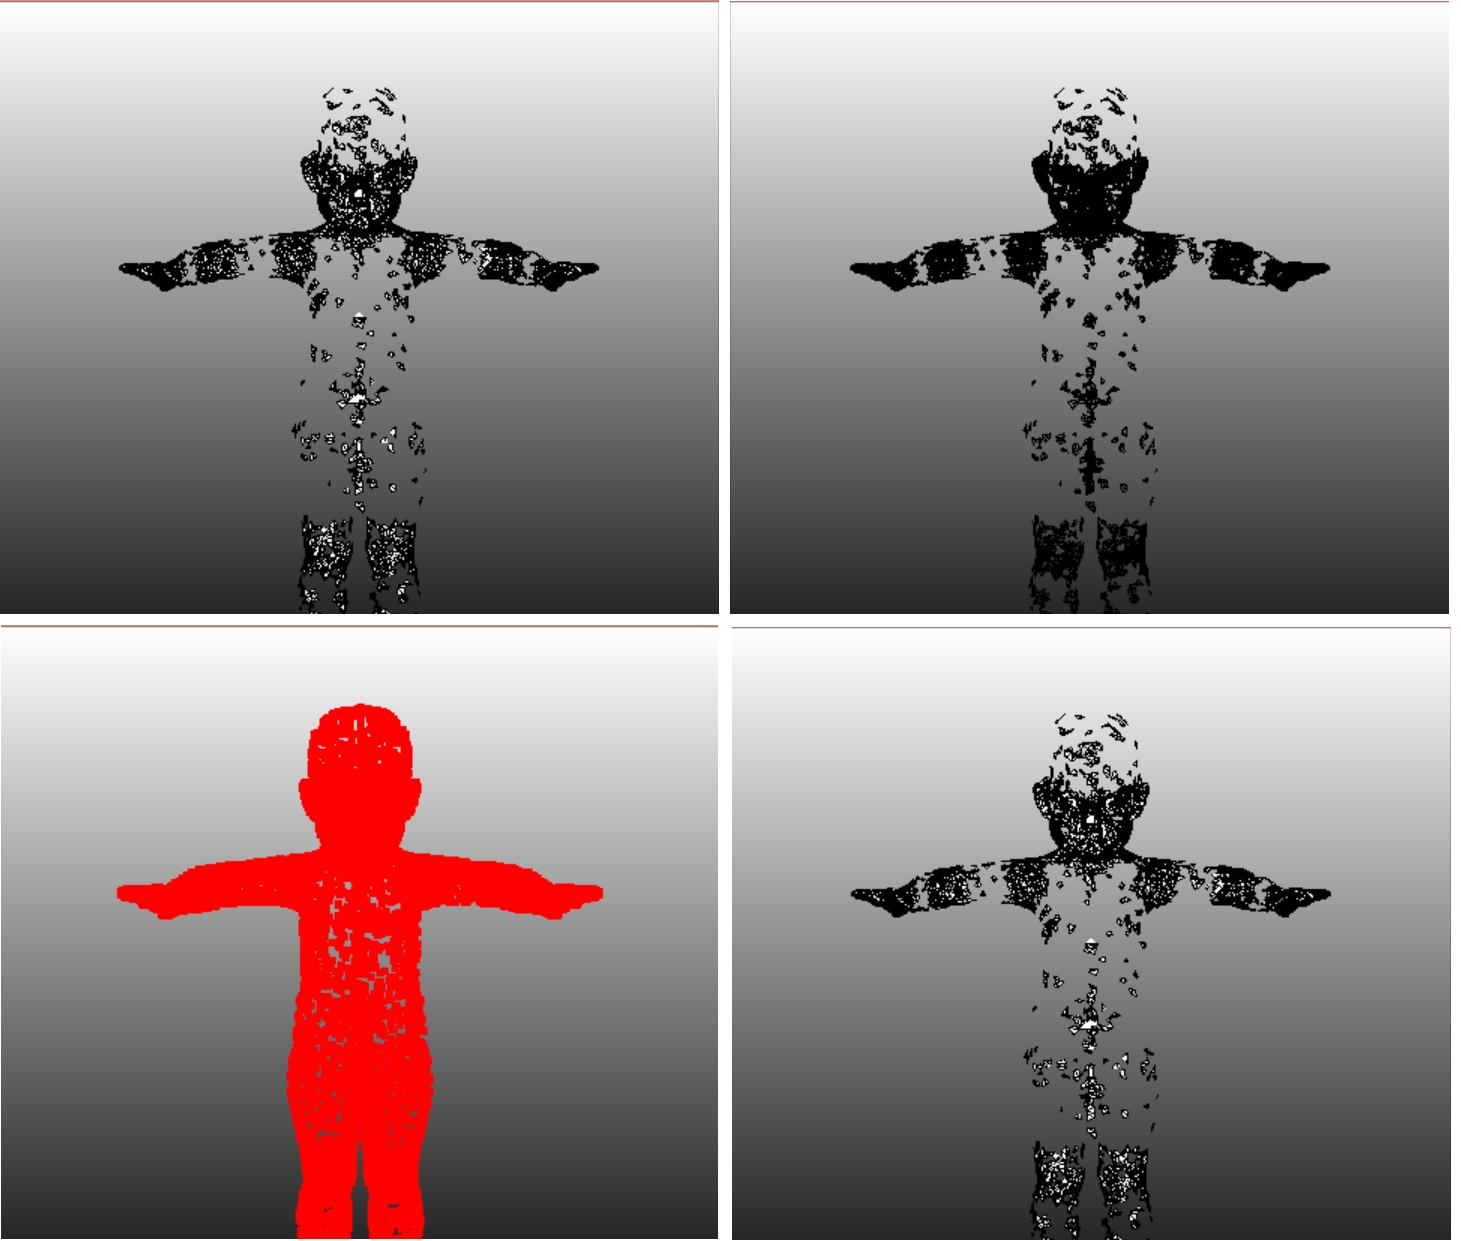
\includegraphics[width=120mm]{bb 10.jpg}\\
  Fig 4. $\alpha=10\hspace{0.15cm}$facets, edges, points and tetrahedra
\end{figure}

\begin{figure}[h]
  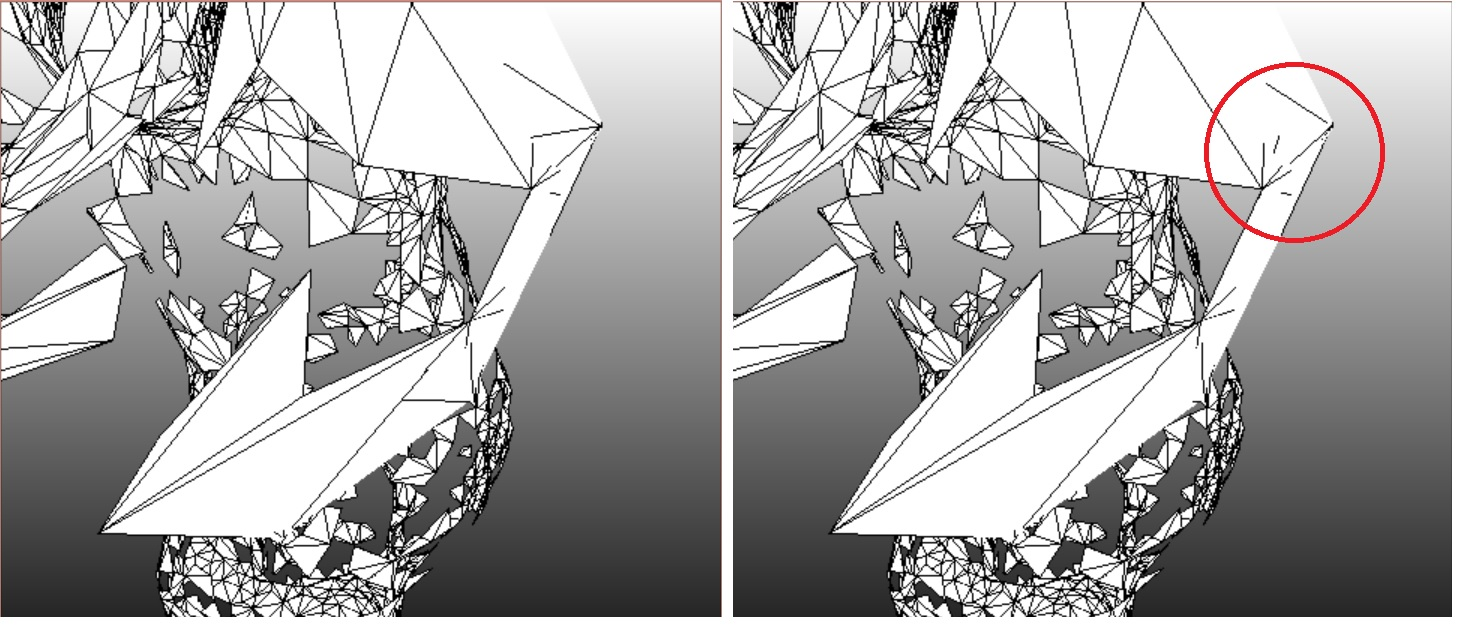
\includegraphics[width=140mm]{differece_btw_facetAndtetra.jpg}\\
  Fig 5. $\alpha=10000000 \hspace{0.15cm}$The difference between facets and tetrahedra
\end{figure}



\section{Known bugs/limitations}
I used the qh.setvoronoi.all() here to get the center of the circumsphere of tetrahedrons. It was confusing that whether the center is calculated from 4D, since the coordinate of the center was consists of four component. But for the every coordinate of center, the 4th component was same with the 1st component so I understood it as a redundant and the qh.setvoronoi.all() returns the coordinate of center in 3D.\\
The circumsphere does great work to find the more exact shape of given scattered point in $\mathbb{R}^3$. It is really awesome.
I completed the edge part in Delaunay() and alpha-shpae(). I want you to check it professor.  

\bibliographystyle{plain}
\bibliography{report}

\end{document}


